
\chapter{Iteration-Fusing Conjugate Gradient}
\label{chap:ifcg}

\newcommand{\MAXPERF}{42\%}
\newcommand{\AVERAGEPERF}{13\%}
\newcommand{\MAXLOC}{81\%}
\newcommand{\AVERAGELOC}{28\%}

%\newcommand{\cmark}{\ding{51}}%
%\newcommand{\xmark}{\ding{55}}%


In the last few years processor clock frequencies have stagnated, while exploiting
Instruction-Level Parallelism (ILP) has already reached the point of diminishing returns.
Multi-core designs arose as a solution to overcome some of the technological constraints
that uniprocessor chips have, but they exacerbated some others as a counterpart.
Multi-core architectures can potentially provide the desired performance by exploiting
Thread Level Parallelism (TLP) of large scale parallel workloads on chip. Such large
amount of parallelism is managed by the software, which means that the programmer needs to
implement highly efficient and architecture-aware parallel codes to achieve the expected
performance. This is obviously much harder than programming a uniprocessor chip, which is
commonly referred as the \emph{Programmability Wall}~\cite{Chapman:2007multicore}.
Moreover, dealing with this wall will be even harder in the near future with the arrival
of many-core systems with tens or hundreds of heterogeneous cores and accelerators
on-chip.

Threading is the most common way to program multicore processors. POSIX threads
(Pthreads)~\cite{Butenhof:1997:PPT:263953} and OpenMP~\cite{Chapman:2007:UOP:1370966} are
two of the most common programming models to implement threading schemes.  Additionally,
MPI~\cite{Nagle:2005:MCR:1239662.1239666} can be incorporated to threading codes to handle
parallelism in a distributed memory environment.  However, to develop efficient threading
codes can be a really hard job due to the increasing amount of concurrency handled by
many-core processors and the current trend towards more heterogeneity within the chip.
Synchronization points are often needed in threading codes to control the data flow and to
enforce correctness.  However, the cost of these schemes increases with the amount of
parallelism handled on chip, seriously hurting performance due to issues like load
imbalance or NUMA effects.  Also, relaxing synchronization costs often involves
significant programming efforts as it requires the deployment of complex and application
specific mechanism like thread pools.

Task
parallelism~\cite{Fatahalian:2006:SPM:1188455.1188543,Blumofe1995,Bellens:SC2006,Ayguade:2009:DOT:1512157.1512430,Tzenakis:2012:BBD:2370036.2145864,Jenista:2011:OSO:2038037.1941563,Planas:2009:HTP:1572226.1572233,Duran:PPL2011}
is an alternative parallel paradigm where the load is organized into tasks that can be
asynchronously executed.  Also, some task-based programming models allow the programmer to
specify data or control dependencies between the different tasks, which allows
synchronization points relaxation by explicitly specifying the data involved in the
operation~\cite{Jenista:2011:OSO:2038037.1941563,Ayguade:2009:DOT:1512157.1512430,Tzenakis:2012:BBD:2370036.2145864,Duran:PPL2011}.

The task-based execution model requires to track the dependencies among tasks, which can
be explicitly specified by the programmer
~\cite{Jenista:2011:OSO:2038037.1941563,Zuckerman:2011:UCP:2000417.2000424} or dynamically
handled by an underlying runtime
system~\cite{DuranIJPP09,Tzenakis:2012:BBD:2370036.2145864,Duran:PPL2011}.  When
dependencies are detected among tasks, a deterministic execution order is applied by the
runtime system to enforce correctness.  In this way, all the potential parallelism of the
code is exposed to the runtime system, which can exploit it depending on the available
hardware.  Additional optimizations like load balancing or work
stealing~\cite{Blumofe1995,Duran:PPL2011} can be applied at the runtime system layer
without requiring any platform-specific consideration from the programmer. 

The potential of task-based programming models is expected to be significant in a wide
range of areas.  In this Chapter we show our task-based implementation of the PARSEC
benchmarks (PARSECSs).  Our objective is to provide an evaluation framework for task-based
parallel models with data dependence tracking.  This combination allows programmers to
exploit parallelism in applications that is not feasible, or require tremendous effort
from the programmers part, when using other parallel models.  The PARSEC benchmark suite 
is a suitable test best, since the applications include are not restricted to small 
kernels.  Instead, the diverse set of workloads and computing domains covered offers the
opportunities for task parallel and dataflow based models to exploit such parallelism.  

These emerging parallelization paradigms offer a more diverse test bed than typical
fork-join models with barrier synchronization.  This allows us to better understand the
impact of manufacturing variability on modern parallel workloads.  Moreover, task-based
programming models are coupled with runtime systems, which deal with load balancing,
dependence tracking, thread synchronization and data allocation.  These are all necessary
tools to deliver good performance and should already be able to deal with manufacturing
variability to some extend.  In this work we don't aim to simply expose manufacturing
variability, our goal is to effectively mitigate it.  By studying its impact on a state-of-the-art 
runtime system, we can offer a solution that is relevant and significant by today's
standards.    

\section{Benchmarking in HPC}
\label{sec:hpc_benchmarking}

Other studies exist that compare parallel programming models in the literature.  Although
these studies do not focus on task parallelism, they employ benchmarks and similar
methodology to evaluate their target models.  \cite{Coarfa:2005:EGA:1065944.1065950} study
and compare the performance of UPC and Co-array Fortran, two PGAS languages.  They use
select benchmarks from the NAS benchmark suite.
\cite{Appeltauer:2009:CCP:1562112.1562118} use microbenchmarks to measure and compare the
performance of 11 context-oriented languages.  Their study shows that they all often
manifest high overheads.


Although all the works we mention try to evaluate various programming models, in terms of
performance, and some times on usability and versatility, they are all limited to small
kernels or even just micro-benchmarks.  We find that this approach is not sufficient to
give us an insight on how a model will impact actual large-scale applications.
\cite{Karlin:2013:ETE:2510661.2511433} use a proxy application in their work to evaluate a
number of different programming models (OpenMP, MPI, MPI+OpenMP, CUDA, Chapel, Charm++,
Liszt, Loci).  Their approach however is limited to only one application.  Different
application domains can be very different, and may require different parallelization
techniques to get good scalability and performance.  A programming model could fail to
even provide a way to express a parallelization scheme, let alone deliver performance.  It
is important to have an in depth understanding of a models behavior and limitation in
order to make an educated decision whether research should direct its efforts to adopt
and further expand it. 


Pipeline parallelism has been the subject of study in some recent studies.  This
programming idiom is found often in streaming and server applications and goes far beyond
the HPC domain.  \cite{Lee:2013:OPP:2486159.2486174} propose an extension to the Cilk
model, for expressing pipeline parallelism on-the-fly, without constructing the pipeline
stages at their dependencies a priori.  It offers a performance comparison between the
proposed model, Pthreads and Thread Building Blocks (TTB) for three PARSEC benchmarks,
ferret, dedup and x264.

This trend of using microbenchmarks and kernel application is also followed when
evaluating other aspects of HPC, apart from parallel programming models, such as emerging
microarchitectures, novel load-balancing techniques and scheduling policies, etc.  The
SPEC CPU2006~\cite{Henning:2006:SCB:1186736.1186737} and SPEC
CPU2017~\cite{Bucek:2018:SCN:3185768.3185771} are benchmark suites designed to evaluate
processor architectures.  However, although the included workloads are fitting for
processor design evaluation, they are not representative of larger, more complex
applications that are run in today's large computer systems.  The PARSEC benchmark
suite~\cite{bienia2008} on the other hand is composed by applications from varying
computing domains, but are also common problems run on HPC systems.  Both SPEC and the
PARSEC however, are implemented using the most basic of parallel programming models, like
Pthreads.  Such programming models, although expressive enough to exploit the available
parallelism, offer little insight into how these applications interact with more
sophisticated programming models, which may have a dedicated runtime system to deal with
workload management and synchronization.  In this work we implement a variation of the
PARSEC benchmarks suite, the PARSECSs, using OMPSs/OpenMP 4.0 task directives and dataflow
relations.  Our implementation uses the most common features between contemporary
task-based models, so they can be easily ported.  Using task parallelism allows us to
implement more complex and efficient parallel programming paradigms, like pipelines.  In
this work, we will be using the PARSECSs to evaluate our runtime and job management
solutions to mitigating the manufacturing variability.
 

\section{The PARSEC Benchmark Suite}
\label{sec:parsec}

\begin{table*}[!t]
	\centering
	\scriptsize
	\caption{\PARSEC{} Benchmark Suite}
	\begin{tabular}{|l|p{6cm}|p{3cm}|p{1cm}|}
	\hline
	\textbf{Benchmark} & \multicolumn{1}{|c|}{\textbf{Description}} & \multicolumn{1}{|c|}{\textbf{Native input}} & \multicolumn{1}{|c|}{\textbf{LOC}}\\
	\hline \hline
	blackscholes & Intel RMS benchmark. It calculates the prices for a portfolio of European options analytically with the Black-Scholes partial differential equation (PDE). & 10,000,000 options & 404 \\ \hline
	bodytrack & Computer vision application which tracks a 3D pose of a marker-less human body with multiple cameras through an image sequence. & 4 cameras, 261 frames, 4,000 particles, 5 annealing layers & 6,968\\ \hline
	canneal & Simulated cache-aware annealing to optimize routing cost of a chip design. & 2,500,000 elements, 6,000 temperature steps & 3,040\\ \hline
	dedup & Compresses a data stream with a combination of global compression and local compression in order to achieve high compression ratios. & 672 MB data & 3,401\\ \hline
	facesim & Intel RMS workload which takes a model of a human face and a time sequence of muscle activation and computes a visually realistic animation of the modeled face. & 100 frames, 372,126 tetrahedra & 34,134\\ \hline
	ferret & Content-based similarity search of feature-rich data such as audio, images, video, 3D shapes, etc. & 3,500 queries, 59,695 images database, find top 50 images & 10,552\\ \hline
	fluidanimate & Intel RMS application uses an extension of the Smoothed Particle Hydrodynamics (SPH) method to simulate an incompressible fluid for interactive animation purposes. & 500 frames, 500,000 particles & 2,348\\ \hline
	freqmine & Intel RMS application which employs an array-based version of the FP-growth (Frequent Pattern-growth) method for Frequent Itemset Mining (FIMI). & 250,000 HTML documents, minimum support 11,000 & 2,231\\ \hline
	raytrace & Intel RMS workload which renders an animated 3D scene. & 200 frames, 1,920$\times$1,080 pixels, 10 million polygons & 13,751\\ \hline
	streamcluster & Solves the online clustering problem. & 200,000 points per block, 5 block & 1,769\\ \hline
	swaptions & Intel RMS workload which uses the Heath-Jarrow-Morton (HJM) framework to price a portfolio of swaptions. & 128 swaptions, 1,000,000 simulations & 1,225\\ \hline
	vips & VASARI Image Processing System (VIPS), which includes fundamental image processing operations. & 18,000$\times$18,000 pixels & 127,957\\ \hline
	x264 & H.264/AVC (Advanced Video Coding) video encoder. & 512 frames, 1,920$\times$1,080 pixels & 29,329\\ \hline 
	\end{tabular}
	\label{tab:parsec}
	\vspace{1cm}
\end{table*}

With the prevalence of many-core processors and the increasing relevance of application domains that do not belong to the traditional HPC field, 
comes the need for programs 
representative of current and future parallel workloads. 
The \PARSEC{}~\cite{Bienia:PhD2011} features state-of-the art, 
computationally intensive algorithms and very diverse workloads from different areas of computing.
\PARSEC{} is comprised of 13 benchmark programs. 
The original suite makes use of the Pthreads parallelization model for all these benchmarks, 
except for \texttt{freqmine}, which is only available in OpenMP. 
The suite includes input sets for native machine execution, which are real input sets.
Table~\ref{tab:parsec} describes the different benchmarks included in the suite along with their respective native input and the lines of code 
(LOC) of each application.
We apply tasking parallelization strategies to 11 out of its 13 applications: \texttt{blackscholes}, \texttt{bodytrack}, \texttt{canneal}, \texttt{dedup}, \texttt{facesim}, \texttt{ferret}, 
\texttt{fluidanimate}, \texttt{freqmine}, \texttt{streamcluster} and \texttt{swaptions} and \texttt{x264}. 
We leave 2 applications out of this study: \texttt{raytrace} and \texttt{vips}.
\texttt{Vips} is a domain specific runtime system for image manipulation. 
Since vips is a runtime itself, it is not reasonable to implement it on top of another runtime system. 
Therefore we do not include this code in our evaluations. 
\texttt{Raytrace} code has the same extension as 
\texttt{ferret}, \texttt{facesim} and \texttt{bodytrack} and the same parallel model as \texttt{blackscholes}~\cite{Cook:2013:HEC:2508148.2485949}.
Therefore, since it does not offer any new insight, we do not consider the \texttt{Raytrace} code in this work.
 
We have a preliminary task-based implementation of the \texttt{x264} encoder, which scales up to 14x on a 16-core machine, the same as the Pthreads version.  
Since we just emulate the same parallel model as the original Pthreads version and obtain the same performance, we do not include this code in the results Section as it provides no insight.




\label{sec:parsecss_implementation}
\section{Application Parallelization}
In this Section we discuss how the \PARSEC{} applications are parallelized in Pthreads/OpenMP2.0 and how they can be implemented efficiently 
using a task-based approach.  When possible, we exploit dataflow relations in order to take advantage of implicit synchronization 
(as described in Section~\ref{sec:task-model}). If it is not possible we use conventional synchronization primitives such as locks,
atomics and barriers.

\paragraph{\textbf{Blackscholes}}
This application solves a Black-Scholes Partial Differential Equation~\cite{RePEc:ucp:jpolec:v:81:y:1973:i:3:p:637-54} to calculate the
prices for a portfolio of ten million European options.

\begin{figure}[t!]%
	\center
	\includegraphics[width=0.5\columnwidth]{ifcg/figures/blackscholes_taskgraph}%
	\caption{Task-graph of blackscholes application.  No dependencies exit between tasks,
only barrier synchronization between iterations.}
	\label{fig:blackscholes_tg}%
	\vspace{.5cm}
\end{figure}

\paragraph{\textit{Pthreads}} This version simply divides the portfolio into
work units by the number of available threads, and stores them into the
\texttt{numOptions} array. Each thread calculates the prices for its
corresponding options and waits in a barrier until all the threads have
finished executing. The algorithm is run multiple times to obtain the final
estimation of the portfolio.


\paragraph{\textit{Task-based}} In the case of the task-based version, we
divide the work into units of a predefined block size. This block size allows
having much more task instances than threads, which implies a much better load
balance, as this is an embarrassingly parallel application with no dependencies
among tasks in the same run.  A task graph of the task-based implementation is
shown in figure \ref{fig:blackscholes_tg}.  We can see that this is an embarrassing
parallel application with only barrier synchronization between iterations of the 
main loop.  No data dependencies exist between tasks.
For all the task graphs shown in this document
we use smaller workloads than the ones used for evaluation.  This way it's easier
to read the task graphs.  For example in figure \ref{fig:blackscholes_tg} there are
four tasks per iteration, but this is easily configurable to hundreds or thousands 
of tasks.  Such is the case of the native workloads used for the evaluation of our 
implementations.



\begin{figure*}[ht!]
	\vspace{1cm}
	\centering
  \begin{subfigure}{0.9\textwidth}
		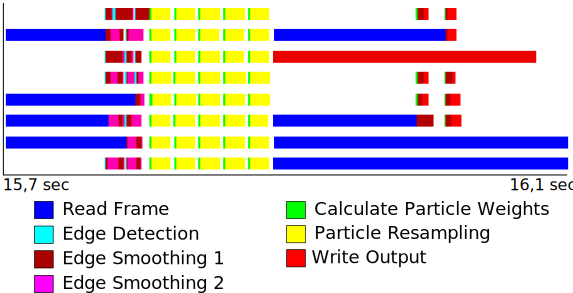
\includegraphics[width=\textwidth]{ifcg/figures/bodytrack-ompss-native-8-2dp_tasks_pthreads}
		\caption{Trivial Task-based Strategy}
	\label{fig:bodytrack-2dp_tasks-trace_pthreads}
  \end{subfigure}%
\\
\vspace{1cm}
\begin{subfigure}{0.9\textwidth}
		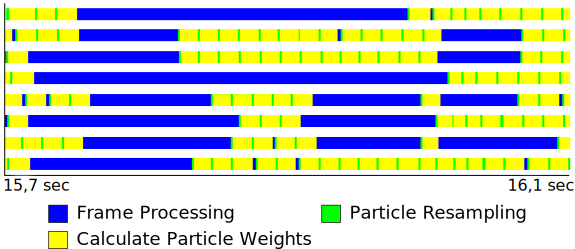
\includegraphics[width=\textwidth]{ifcg/figures/bodytrack-ompss-native-8-2dp_tasks_ompss}
		\caption{Optimal Task-based Strategy}
	\label{fig:bodytrack-2dp_tasks-trace_ompss}
  \end{subfigure}
	\caption{Parallel execution of Pthreads and task-based versions of \texttt{bodytrack} on an 8-core machine and native input size. Different parallel regions correspond to different colors.  White gaps in the figure, represent idle time.}%
	\label{fig:bodytrack-2dp_tasks-trace}%
\end{figure*}

\paragraph{\textbf{Bodytrack}}
Computer vision application that tracks a marker-less human body using multiple cameras
through an image sequence.  The application employs an annealed particle filter to track
the body using edges and the foreground silhouette as features of interest.

\begin{figure}[t!]%
	\center
	\includegraphics[width=\columnwidth]{ifcg/figures/bodytrack_taskgraph}%
	\caption{Task-graph of bodytrack application.  Edges show task data dependencies.}
	\label{fig:bodytrack_tg}%
	\vspace{.5cm}
\end{figure}



\paragraph{\textit{Pthreads}} \texttt{Bodytrack} applies the same algorithm on each frame
of the image sequence to track the different poses of the body.  The human body is modeled
as a tree-based structure, consisting of 7 conic cylinders.  It reads 4 images taken from
several cameras to capture a scene from 4 different angles, thus each frame consists of
these 4 images.  These images are read and encoded to a single data structure.  For each
frame, \texttt{bodytrack} extracts the edges and silhouette features for each of these 4
images.
In this feature extraction stage we have 3 different kernels.
\begin{enumerate}
	\item \textbf{Edge detection}: Gradient based edge detection.
	\item \textbf{Edge smoothing (phase 1)}: Gaussian filter used to smooth edges applied on array rows.
	\item \textbf{Edge smoothing (phase 2)}: Gaussian filter used to smooth edges applied on array columns.
\end{enumerate}
Afterwards, \texttt{bodytrack} goes through an annealed particle filter stage, which
consists of M annealing layers over a set of N particles.  The particles are multi-variate
configurations of the state and location of the tracked body.  Given the image features,
the particles are assigned weights, which increase or decrease the chance that a particle
represents a body part.  N particles are then chosen, depending on the probability
dictated by their weights.  Random noise is added to this set of particles, creating a new
set.  This process is repeated for all annealing layers. \texttt{Bodytrack} then picks one
of the M configurations, the one which has the highest weighted average.  This process has
two parallel kernels.
\begin{enumerate}[resume]
	\item \textbf{Calculate particle weights}: Computes weights for the particles, using the edges and silhouette produced from the previous stages.
	\item \textbf{Particle Resampling}: Adds Gaussian random noise to the particles, thus creating a new set of particles.
\end{enumerate}

In the case of Pthreads, the 4 images of a frame are read and processed in parallel using
one thread per image.  The Pthreads implantation is limited by the 4 images it can process
concurrently, while there is no other candidate work at this point.  A specific
asynchronous I/O implementation is required to read the files in parallel. Then, the
features extraction stage is executed using all the available threads, with a
synchronization barrier at the end of each phase. The same structure is followed in the
annealed particle filter stage, with two barriers at the end of each phase. Between the
two stages, serial code has to be executed, which leaves only one thread busy and the rest
idle.  Finally, the output results are written sequentially in one file.   


\paragraph{\textit{Task-based}} In the case of the task-based version, we adopt a more coarse grain approach. 
We do not parallelize the feature extraction stage, instead we 
taskify the whole frame processing, allowing concurrent execution of all frames. 
%Given enough frames to process, all threads can remain busy,
%which is not the case with the Pthreads version.
The parallel kernels of the annealed particle filter stage are taskified in our version, and synchronization is achieved
by dataflow annotations.  Figure \ref{fig:bodytrack_tg} shows a task graph of our implementation.  The directed edges show the
dependencies between the different tasks, which dictate the execution order of the tasks.
Each frame needs to be written when calculations are completed. In our version we can do this asynchronously while the threads are
busy with the processing stage of another frame.  Thus, output I/O is effectively overlapped with computation stages.


{Figure \ref{fig:bodytrack-2dp_tasks-trace} shows parallel executions of two different task-based implementations: 
The first one just mimics the Pthreads behavior (\ref{fig:bodytrack-2dp_tasks-trace_pthreads}) and the second is an optimal task-based implementation (\ref{fig:bodytrack-2dp_tasks-trace_ompss}).  
Different colored boxes represent different task types, as well the duration of that task type on each core. In both cases, the white gaps denote the time each thread spends idle.  
Both figures show the same duration for each execution. In the optimal version, all functionality is implemented within the frame-processing task, thus 
execution time for read-frame, edge-detection and edge-smoothing is represented with blue color (frame-processing).  
Tasks particle-resampling and calculate-particle-weights are also implemented as nested tasks. 
They are displayed with different colors (green and yellow respectively).  
We can observe that the Pthreads-like version suffers
from greater idle time compared to its optimal task-based counterpart. 
Work is distributed more efficiently in the optimal implementation
by processing different frames concurrently. 
This allows us to overlap I/O and serial code segments of one with available work from another one.
       
%To illustrate this point, Figure~\ref{fig:bodytrack-2dp_tasks-trace} shows an execution of \texttt{bodytrack} for two different frames. The x-axis represent time and the y-axis represent the cores where the execution takes place. 
%For example, a pixel of color blue in the (x,y) point means that at the instant x the core y is running the task codified by color blue. The red, dark red and green are tasks performing edge detection and edge smoothing, respectively.  
%The yellow color represents the task writing the output file. 
%Light green and magenta are the tasks that calculate particle weights and re-sample the particles. Light blue color annotates the idle time or sequential code execution. 
%%
%We can see how the task that writes the output file for frame N-1 (in yellow) is overlapped by the three first computation tasks of frame N, which does not happen in the Pthreads version of the code.
%This overlapping is the main source of performance gains archived by using the dataflow task-based paradigm with \texttt{bodytrack}. 
%Section~\ref{sec:evaluation} reports these improvements in detail.

\paragraph{\textbf{Canneal}}
This kernel uses a cache-aware simulated annealing~\cite{Banerjee:1994:PAV:185340} to
optimize routing cost of a chip design.  \texttt{Canneal} progressively swaps elements
that need to be placed in a large space, eventually converging to an optimal solution. The
problem is stored as a list with routing costs between nodes. 

\begin{figure}[t!]%
	\center
	\includegraphics[width=.8\columnwidth]{ifcg/figures/canneal_taskgraph}%
	\caption{Task-graph of canneal application.  Only barrier synchronization among tasks.}
	\label{fig:canneal_tg}%
	\vspace{.5cm}
\end{figure}

\paragraph{\textit{Pthreads}} This version compares random element pairs of the graph
concurrently and swaps them until it converges to an optimal solution.  No locks are used
to protect the list from concurrent accesses/writes, but  swaps are done atomically
instead. However, the evaluation of the elements to be swapped is not atomic.  This means
that disadvantageous swaps may occur, which will require the algorithm to eventually swap
them again.  This method has provided better results than the alternative algorithm with
locks~\cite{bienia2008}.

\paragraph{\textit{Task-based}} Our task-based version follows the same paradigm.  Several
tasks are spawned without any dependencies between themselves. We use the same atomics as
with the Pthreads version.  Since tasks work with an arbitrary number of list elements, it
is not possible to describe which elements of the list a task is going to randomly access. 
In the task graph in figure \ref{fig:canneal_tg} it is clear that there are no data dependencies.
Synchronization is only achieved through the use of barriers.

We also try an alternative fine grain implementation, where a task is spawned for each
random pair of list elements.  This would allow the runtime to know if two tasks are
working on the same list of elements. However this implementation implied fine-grain
tasks. Each task would merely do a single swap between two list elements.  The overhead of
the dynamic scheduling is a problem in this scenario.  A more complex but more efficient
solution is suggested by Symeonidou et al.~\cite{Symeonidou:2013:DDR:2488551.2488558} with
the use of memory regions.  Adopting this method in a task-based model would allow the
programmer to describe parts of the list (or other pointer based data structures) and
express dataflow relations as abstract memory regions.  This solution also implies
fine-grain tasking and is not evaluated at the Symeonidou's work. 

\begin{figure}[t!]%
	\center
	\includegraphics[width=.4\columnwidth]{ifcg/figures/dedup_taskgraph}%
	\caption{Task-graph of dedup application.  Data dependency edges force the correct order
of writting the data chunks to the output.}
	\label{fig:dedup_tg}%
	\vspace{.5cm}
\end{figure}


\paragraph{\textbf{Dedup}}
The \texttt{dedup} kernel is used to compress data streams using local and global
compression to achieve higher compression rates.  This method is called
deduplication~\cite{Quinlan:2002:ABP:1083323.1083333}.

\paragraph{\textit{Pthreads:}}
Dedup is parallelized using a pipeline model with the following stages:
\begin{itemize}
  \item \textbf{Fragment}:  First, the data-stream is read and partitioned at fixed positions into coarse grain data chunks. Each chunk can be processed individually by the rest of the stages. This stage is executed on a single thread.
  \item \textbf{Fragment Refine}:  A new data chunk initiates the second pipeline stage, where it is further partitioned into smaller fine-grain
	chunks.  The portioning is done by using the Rolling-fingerprint algorithm.  
  \item \textbf{Deduplication}:  This stage eliminates duplicate fine-grain chunks.  Unique chunks are stored in a hash-table.
	Locks are used here to protect	each bucket from concurrent accesses.
  \item \textbf{Compress}:  At this stage chunks are compressed in parallel.  Identical chunks are compressed only once as duplicates are removed 
	at the deduplication stage.
  \item \textbf{Reorder}:  This stage writes the final compressed output data to a file.  It writes only unique chunks' compressed data and for the
	duplicates it stores their hash values.  However this stage needs to reorder the data chunks as they are received
	to match the original order of the uncompressed data.
\end{itemize}

The Pthreads version maintains a queue and a thread pool dedicated to each stage.  When a
chunk becomes available at one stage, it is moved to the queue of the next stage.  Each
stage polls at its queue for available chunks to process. The reorder stage is done
sequentially with a devoted thread that can be in an idle loop waiting for previous stages
to finish.  Each thread pool  comprises by a number of threads equal to the number of
available cores.  The only exceptions are \texttt{Fragment} and \texttt{Reorder} stages,
which are served by a single thread each.

%\begin{figure}[ht!]%
%	\centering
%	\begin{lstlisting}
%void Fragment{
%  ...
%  while ( chunk = read_bytes() ) {
%		chunks[nCChunks][0] = chunk;
%		#pragma omp task inout(chunks[nCChunks]) 
%		Fragment(chunks[nCChunks]);
%		#pragma omp task inout(chunks[nCChunks])
%		WriteOutput(outfile, chunks[nCChunks]);
%		nCChunks++;
%		break;
%  }
%  #pragma omp taskwait
%	...
%}
%	\end{lstlisting}
%	\caption{Dedup task-based implementation pseudocode of the \texttt{Fragment} stage.}%
%	\label{lst:dedup-ompss}%
%\end{figure}

\begin{figure}[!t]%
	\centering
	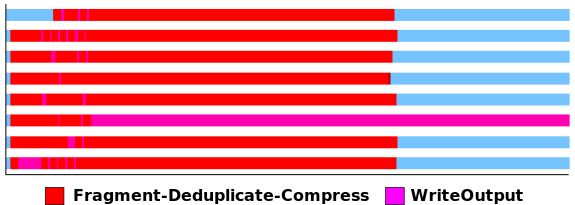
\includegraphics[width=0.9\columnwidth]{ifcg/figures/dedup-ompss-native-8-2dp_tasks}%
	\caption{Parallel execution of the task-based version of \texttt{dedup} on an 8-core machine and native input size. Different task types correspond to different colors.}%
	\label{fig:dedup-2dp_tasks-trace}%
	\vspace{.5cm}
\end{figure}


\paragraph{\textit{Task-based}}
In our implementation we taskify each pipeline stage and express data dependencies using static arrays and dataflow relations, one for each pipeline stage.
\texttt{FragmentRefine} however partitions the data chunks into very fine grain segments, ranging from a few hundreds to thousands. For such granularity,
our approach suffers from high overheads due to dynamic schedulnig overhead. 
The same is observed in~\cite{Vandierendonck:2013:DSP:2503210.2503233}, where 
an alternative approach is adopted. In their approach, two pipelines are identified: The outer pipeline, consisting of stages \texttt{Fragment}, \texttt{InnerPipeline}
and \texttt{Reorder}. The inner pipeline consists of \texttt{FragmentRefine}, \texttt{Deduplicate} and \texttt{Compress}.  To reduce the dynamic scheduling overhead,
they merge together \texttt{Deduplicate} and \texttt{Compress}. By doing so, the available parallelism is limited, but still there is enough work not to harm performance
and scalability. In our approach, we merge together the inner pipeline, creating one sequential function, exploiting only the parallelism available in the outer pipeline.
Even in this scenario, the available parallelism is still abundant, since the application is bound by the writing of the output file, which is sequential.  
Figure~\ref{fig:dedup-2dp_tasks-trace} shows a trace of the task-based version.  We can see that communication stage (in yellow) is effectively overlapped with the computation stage (in red), however,
there is not enough work to keep all the threads finish, until the end of the execution.

Furthermore, we modify the \texttt{Reorder} stage, by replacing it with a simple stage where the chunk is simply written to file (\texttt{WriteOutput}).
Using dataflow relations and a shared output resource between the \texttt{WriteOutput} tasks, we ensure that chunk \texttt{N-1} will be written before chunk \texttt{N}. 
Thus, we do not need to reorder data chunks in this task type.  Moreover, the scheduler makes sure chunks are written as soon as they become available by the \texttt{InnerPipeline} task, an improvement
over the Pthreads version, where \texttt{Reorder} instances need to idle wait until all previous chunks ones have been written.  
Figure \ref{fig:dedup_tg} shows the dependencies among tasks.  We can observe that \texttt{WriteOutput} tasks will be run in the correct
order, as soon as their dependencies are resolved.
Another difference between the two versions, is that Pthreads 
oversubscribe threads to cores for each pipeline stage, while in our implementation we only assign one thread to each core.


\paragraph{\textbf{Facesim}}
Computes a visually realistic human face animation by simulating the underlying physics.  As input it uses a 3D model of a human face 
containing both a tetrahedra mesh and triangulated surfaces for the flesh and bones, respectively. Additionally it uses 
a time sequence of muscle movement \cite{Sifakis:2005:ADF:1073204.1073208}.

\paragraph{\textit{Pthreads}}
The application statically decomposes the original tetrahedron mesh into smaller partitions, equal to the number of available threads.
%The boundaries of the partitions are replicated to avoid synchronization. The trade-off is redundant computations. For the bones, they 
%are employed serially. 
There are three main parallel kernels:
\begin{itemize}
  \item \textbf{Update State}: Calculates the steady properties of the mesh, constrains like stress and stiffness.  
%This is done by solving a nonlinear system of equationsusing the Newton-Rhapson method.  
  \item \textbf{Add Forces}: Computes the force contribution between vertices acting on the 3D model.
  \item \textbf{Conjugate Gradient (CG)}:  An iterative method that solves the linear system produced by the 
other two previous kernels and find the final displacement of the vertices for the current frame.
\end{itemize}

\texttt{Update\_State} and \texttt{Add\_Forces} kernels consist of one and two parallel loops respectively, while \texttt{CG} has three. 
Synchronization between loops and kernels is achieved by barriers.  The corresponding force computations from the skeleton are also done 
in \texttt{Update\_State} and \texttt{Add\_Forces}, but after the parallel computations on the tetrahedra mesh have been made. 
In Pthreads a master thread is assigning work to all threads in a round-robin fashion through a queuing system.  Each thread maintains 
its private queue, which is protected by locks.

%\begin{figure}[!t]%
%	\centering
%	\includegraphics[width=0.8\columnwidth]{figures/facesim-ompss-native-8-2dp_tasks}%
%	\caption{Parallel execution of the task-based version of \texttt{facesim} on an 8-core machine while simulating a frame. 
%	Different task types correspond to different colors, while idle time is represented in light blue color.}%
%	\label{fig:facesim-2dp_tasks-trace}%
%\end{figure}

\paragraph{\textit{Task-based}}
In the task-based version, the application level queuing system is completely replaced by the OmpSs runtime.  In our initial implementation 
all parallel loops are taskified. 
Additionally,  in \texttt{Update\_State} there is a sequential code segment, 
\texttt{Update\_Collision\_Penalty\_Forces}.  
This code segment operates on the bones, while the parallel loop of \texttt{Update State} does so on the tetrahedra.  
By taskifying it and adding dataflow relations between this Section and the following \texttt{Add\_Forces} kernel, we can overlap 
\texttt{Update\_Collision\_Penalty\_Forces} with the rest of \texttt{Update\_State}.


%\edit{In the \texttt{CG} kernel, we managed to remove two out of three barriers, which synchronized the different parallel loops, by using dataflow relations 
%to describe data dependencies.  One barrier could not be removed as it protects the residual calculation at theend of each iteration of the solver, 
%whose value is used to control whether we exit the loop or not.}  
%\edit{This initial implementation suffered from high task creation time in the \texttt{CG} kernel.  Note that this is an issue of OmpSs' runtime, out OpenMP 4.0 task implementation 
%did not manifest this issue.}
To improve performance we refactor tasks' creation in \texttt{CG} by nesting the first task creation loop inside another task.
This enables us to overlap task creation time with computation, which contributes to increase \texttt{Facesim's} task-based implementation performance.  
Although we achieve better scalability than the original code, task creation still imposed overheads. To address this issue
we replace tasks in \texttt{CG} with the OmpSs parallel loops construct (equivalent to the OpenMP one), which implements loop worksharing 
with a task. Even though this approach limits the available parallelism (barrier synchronization, no dataflow annotations), the overhead 
associated to task creation and scheduling is greatly reduced and overall performance improved.

\paragraph{\textbf{Ferret}}
Content similarity search server for feature-rich data~\cite{Lv:2006:FTC:1218063.1217966} like audio, video, images, etc.
The benchmark application is configured for image similarity search.  
%\begin{figure}[t!]%
%	\begin{lstlisting}
%void load() {
%	int i = 0;
%	while( load_image(image[i]) ) {
%		#pragma omp task in(image[i]) out(seg_images[i])
%		seg_images[i] = t_seg(image[i]);
%		#pragma omp task in(seg_images[i]) out(extract_data[i])
%		extract_data[i] = t_extract(seg_images[i]);
%		#pragma omp task in(extract_data[i]) out(vectoriz_data[i])
%		vectoriz_data[i] = t_vec(extract_data[i]);
%		#pragma omp task in(vectoriz_data[i]) out(rank_results[i])
%		rank_results[i] = t_rank(vectoriz_data[i]);
%		#pragma omp task in(rank_data[i]) out(outstream)
%		t_out(rank_data[i], outstream);
%		i++;
%	}
%	#pragma omp taskwait
%}
%	\end{lstlisting}
%	\caption{Ferret ompss implementation}%
%	\label{lst:ferret-ompss}%
%\end{figure}

\begin{figure}[t!]%
	\center
	\includegraphics[width=0.9\columnwidth]{ifcg/figures/ferret_tg}%
	\caption{Task-graph of ferret showing the pipelined execution model.  Edges show data dependencies among different tasks.}
	\label{fig:ferret_tg}%
	\vspace{.5cm}
\end{figure}

\paragraph{\textit{Pthreads}}
Ferret is parallelized using a pipeline model.  A serial query is broken down into 
6 pipeline stages:
\begin{itemize}
  \item \textbf{Load}:  This stage loads an image that is going to be used as a query.
  \item \textbf{Segmentation}:  At this stage the image is decomposed into the different objects displayed on it.
	Different weight vectors are to be assigned on each object to achieve better results.
%	For example if an object is identified as a background it will have a smaller weight
%	than other objects.
  \item \textbf{Extract}:  At this stage a 14-dimensional vector is computed for each object from the segmentation stage, 
														describing features such as color, area, state, etc.
  \item \textbf{Vectorization}:  This is the indexing stage that tries to find a set of candidate images in the database.
  \item \textbf{Rank}:  This stage ranks the results found, using the EMD metric for each query-object's vector
	and the database's image vectors.
  \item \textbf{Output}:  Outputs the result of the ranking stage.  Multiple instances of
	this stage need to run serially, since they all share the same output stream.

\end{itemize}

In the Pthreads version every stage is served by a dedicated thread-pool of N threads each, where N is the number of available cores.
The only exceptions are the \texttt{Load} and \texttt{Output} stages that are executed by a respective single thread.
Each stage polls on its corresponding queue for available work.  When a stage finishes,
it pushes the results to the next stage's queue. 

\paragraph{\textit{Task-based}}
In this version, we implement a variation of this pipeline model. As soon as the first
stage, \texttt{Load}, finds a new image, it spawns all stages of a pipeline for that
image, thus reducing the pipeline to five stages.  We model the dataflow relations between
different stages as simple one dimension arrays, as shown in
Figure~\ref{lst:ferret-ompss}.  Tasks working on different image queries do not share any
dependencies. An exception is task \texttt{t\_out} which shares the same output file
between all pipelines, thus sequential execution is forced between all instances of this
task.  The pipeline stages and dependencies are constructed a priori, which is good enough
for this application, but this is not always the case.
\cite{Lee:2013:OPP:2486159.2486174} proposes a system that can handle dynamic pipeline
creation by constructing a DAG with the stages using indexes and the
\texttt{cilk\_continue} and \texttt{cilk\_wait} keywords.  Indexes are used to define the
different pipeline stages, while \texttt{cilk\_continue} creates a stage that can run once
all previous stages in the same pipeline iteration are done, and \texttt{cilk\_wait}
creates a stage that will wait for its stage counterpart of the previous iteration to
finish.  A strategy based on versioning the dependency objects between the stages has been
proposed~\cite{Vandierendonck:2011:PPG:2001252.2001265}.  Output dependencies are renamed
and privatized, thus the static array for privatization is not required.  

Figure \ref{fig:ferret_tg} shows the task-graph of the \texttt{ferret} application.
Colored nodes denote the concurrent tasks (each color matches a specific task type).
Tasks that have data dependencies are connected by directed edges.  By inspecting the
task-graph we can see a pipeline pattern of execution.  Despite the fact that the
task-based approach does not significantly improve the overall performance, as we can see
in Section~\ref{sec:task_bench_evaluation}, it significantly reduces the effort required
to express the pipeline parallelism, compared its Pthreads counterpart, as it is shown in
Section~\ref{sec:lines} in detail.


\paragraph{\textbf{Fluidanimate}}
This application simulates incompressible fluid interactive animation, using the 
Smoothed Particle Hydrodynamics (SPH) method~\cite{Muller:2003:PFS:846276.846298}.

\begin{figure}[t!]%
	\center
	\includegraphics[width=.6\columnwidth]{ifcg/figures/fluidanimate_taskgraph}%
	\caption{Task-graph of fluidanimate application. Edges represent data dependencies among
tasks}
	\label{fig:fluidanimate_tg}%
	\vspace{.5cm}
\end{figure}

\paragraph{\textit{Pthreads}}
\texttt{Fluidanimate} uses five special kernels which are responsible for rebuilding the
spatial index, computing fluid densities and forces at given points, handling fluid
collisions with the scene geometry and finally updating particle locations The fluid
surface is partitioned and each thread works on its own grid segment.  The kernels are
parallelized as do-all loops, separated by barriers. Moreover, there are cases where these
threads need to update values beyond their partition, which are handled using locks.

\paragraph{\textit{Task-based}}
The task-based implementation follows the same approach, we apply a loop tiling
transformation, for each parallel loop, and taskified each iteration.  
Figure \ref{fig:fluidanimate_tg} show how dependencies form among between tasks.  
Tasks from different loops can run concurrently, as soon as their dependencies are met.
For example we see that the first task of each loop, only requires that the first two tasks
from the previous loop finish their execution to have their dependencies resolved.
We maintain the
same barrier and lock synchronization scheme, using the OmpSs synchronization primitives.

\begin{figure}[t!]%
	\center
	\includegraphics[width=.8\columnwidth]{ifcg/figures/freqmine_taskgraph}%
	\caption{Task-graph of freqmine application.  Edges represent data dependencies among
tasks.}
	\label{fig:freqmine_tg}%
	\vspace{.5cm}
\end{figure}

\paragraph{\textbf{Freqmine}}
Data mining application that makes use of an array-based version of the Frequent Pattern
(FP) growth method for Frequent Itemset Mining~\cite{conf/fimi/GrahneZ03}.

\paragraph{\textit{Pthreads}}
The application uses a compact tree data structure, denoted \emph{FP-tree}~\cite{Han:2000:MFP:335191.335372}, to store information about frequent patterns of the transaction database.  The FP-tree is coupled with a header table, which is a list of database items, sorted by decreasing order of occurrences.
The FP-growth algorithm traverses the FP-tree structure recursively, constructing new FP-trees until the complete set of frequent itemsets is generated.
There are three parallel kernels.  The \texttt{Build\_FP-tree\_header\_table} kernel performs a database scan 
and counts the number of occurrences of each item.  The result is the FP-tree header table.   
\texttt{Build\_Prefix\_tree} kernel performs a second database scan required to build the prefix tree
and the \texttt{Data\_Mining} kernel obtains the frequent itemset information by using the previous two structures.  It creates
an additional lookup table, which allows faster traversals on sparse itemsets.
The original \PARSEC{} benchmark uses OpenMP2.0 for loop parallelization inside each kernel.  

\begin{figure}[ht!]%
	\center
	\includegraphics[width=.6\columnwidth]{ifcg/figures/streamcluster_taskgraph}%
	\caption{Task-graph of streamcluster application.  Edges represent data dependencies among
tasks.}
	\label{fig:streamcluster_tg}%
	\vspace{.5cm}
\end{figure}



\paragraph{\textit{Task-based}}
In our implementation we taskify each iteration. We do not use any dataflow relations in this application, and resolve to 
adopt the locking and barrier synchronization used in the original OpenMP version.
The barrier synchronization is shown in the task graph in figure \ref{fig:freqmine_tg}.

\paragraph{\textbf{Streamcluster}}
Streamcluster is a kernel that solves the online clustering problem. 
It takes a stream of points and then groups them in a predetermined number of clusters with their respective centers.  


\paragraph{\textit{Pthreads}}
Up to 90\% of total execution time is spent in function \texttt{pgain}, 
computing whether opening a new center is advantageous or not.  For every 
new point, function \texttt{pgain} calculates the cost of making it a new center by reassigning some points to it and 
comparing it to the minimum distance $d(x,y) = |{x-y}|^2$ between all points $x$ and $y$.
The result is accepted if found to favor the new center.  Data points are statically partitioned by a given block 
size, which determines the level of parallelism in the application. In the Pthreads version this is equal to the number of
threads. 

\paragraph{\textit{Task-based}}
In our implementation we follow a different decomposition strategy, making the number of tasks independent
of the number of partitions.   
Barriers are employed to synchronize accesses
to a partition in both Pthreads and the task-based implementation. 
In the case of Pthreads, an additional user 
implemented library is used for the barriers. 
This library is not required in the case of the OmpSs implementation, as 
the runtime already has a generic barrier implementation.
A task graph of our task-based implementation and the dependencies among tasks is shown in figure \ref{fig:streamcluster_tg}

\paragraph{\textbf{Swaptions}}
Economics application that uses the Heath-Jarrow-Morton (HJM)\cite{RePEc:ecm:emetrp:v:60:y:1992:i:1:p:77-105} for pricing of a portfolio of swaptions. To calculate prices it employs the Monte Carlo simulation.

\begin{figure}[ht!]%
	\center
	\includegraphics[width=.8\columnwidth]{ifcg/figures/swaptions_taskgraph}%
	\caption{Task-graph of swaptions application.}
	\label{fig:swaptions_tg}%
	\vspace{.5cm}
\end{figure}


\paragraph{\textit{Pthreads}}
The application stores the portfolio into an array. In the Pthreads version, this array is divided by the number of available threads, each thread working on its own part of the array. 

\paragraph{\textit{Task-based}}
We use the exact same strategy, where each task works on a part of the array.  No data dependencies exist between the tasks.
Figure \ref{fig:swaptions_tg} shows the corresponding task graph for the swaptions application.  No dependencies exist between tasks,
synchronization is only achieved through barriers.
%\paragraph{\textbf{x264}}
%An AVC (Advanced Video Coding) video encoder, based on the ITU-T H.264 standard~\cite{H.2642007}.
%It improves over previous video encoding standards at the expense of significantly increased 
%encoding and decoding time.


%The parallel version of x264 extracts parallelism by processing different frames concurrenlty. Initially frames are split in smaller 
%macroblocks of 16x16 pixels.  These macroblocks are processed by a pipeline with a number of stages equal to the number of frames.
%The stages are: \texttt{Read\_frame}, which reads input frames, \texttt{Analyse\_frame}, which creates data dependencies among macroblocks,
%\texttt{Encode\_frame}, which is the encoding state and \texttt{Write\_frame} which writes the encoded frames to the output file.


%The task-based implementation does not use the macroblocks. Instead
%it works on whole frames.  We use two different task types, each spawned for each frame.  The first reads the frame and the second performs the
%three other pipeline stages.  The pipeline stages are synchronized using shared variables. 
 

\section{Programmability}
Different models and languages offer diverse ways to express concepts, such as parallelism or asynchrony.
In this section we evaluate how successful and easy it is to express parallelism using task-based models.  
A good proxy to evaluate how complex a particular implementation is the number of lines of code it takes.
Despite being a metric proposed some decades ago, comparing different programming models in terms of the total number of code lines
is still a valid metric. Indeed, recent publications make an extensive use of it~\cite{Vandierendonck:2011:PPG:2001252.2001265,Dongarra20081}.

%\subsection{Expressiveness}
%\edit{In the Parsec suite we encounter a diverse
%set of parallelization strategies, which however can be grouped into data-parallelism, pipeline parallelism and hybrid between data and pipeline
%parallelism (e.g. \texttt{facesim}).  We were able to express at least the same amount of parallelism in all the 10 benchmarks we used for this study,
%compared to the Pthreads and OpenMP versions.  Additionally, in the cases of \texttt{bodytrack} and \texttt{facesim} we were able to express additional
%parallelism with the use of dataflow annotations and tasks.  Note that in the case of \texttt{dedup}, we adopted a parallelization method with less available
%parallelism than in the case of Pthreads.  We were also able to implement the original Pthreads \texttt{dedup} version but for performance reasons we adopted
%the version with less parallelism.   Section~\ref{sec:implementation} explains this decision in detail.}


%\edit{Although we were able to implement 10 out of the 10 benchmarks, it is possible that we could obtain better results and express additional parallelism in some
%cases, but not with the current standard syntax that OpenMP 4.0 offers.  As discussed in Section \ref{sec:implementation}, the current syntax could benefit from
%extensions that could express data dependencies among irregular and dynamic data structures.  The current OpenMP 4.0 standard is focused on continuous data structures.}

\begin{figure*}[!htbp]
        \centering
        \begin{subfigure}[b]{0.8\textwidth}
                \includegraphics[width=\textwidth]{ifcg/figures/absolute_loc_norm}%
                \caption{Comparison between all source files.}%
                \label{fig:absolute_loc}
                \vspace{0.4cm}
        \end{subfigure}%
				\hfill
        \begin{subfigure}[b]{0.8\textwidth}
        \includegraphics[width=\textwidth]{ifcg/figures/relative_loc_norm}%
        \caption{Comparison between only source files containing parallel code.}%
        \label{fig:relative_loc}%
        \end{subfigure}%
  \caption{Comparison of lines of code between our task-based implementations and the original Pthreads or OpenMP versions.}
        \label{fig:loc_comparison}
\end{figure*}


\subsection{Lines Of Code}
\label{sec:lines}
The reduction of the lines of code (LOC) attests to a more compact and readable code.
%keeping in mind that the actual 
%algorithm complexity remains unchanged.}
In some of our PARSEC task-based implementations, a simple pragma directive replaced application 
specific schedulers, scheduling queues, thread pooling mechanisms and lock synchronization.
We do not change the algorithm in any of the task-based parallel strategy implemented in the PARSEC suite.
Figure~\ref{fig:absolute_loc} shows a normalized comparison between the lines of code of our task-based implementations and the original Pthreads/OpenMP implementations of the PARSEC 3.0 distribution.
The PARSEC 3.0 versions we refer to are always the Pthreads versions, except in the case of \texttt{freqmine} where, since there is no Pthread version available, the OpenMP2.0 version is taken as reference.
We preprocess all source files so that they only contain lines of code relevant to the respective programming model\footnote{PARSEC benchmarks contain mixed serial, Pthreads, OpenMP and TBB source code, and make use of macros to enable conditional compilation for only one programming model at a time.}.
%The LOC column in Table~\ref{tab:parsec} shows the total lines of code for each application, counting all source files.
%Upon careful inspection we can observe that the task-based version requires less lines of code, however parallel code is only a fragment of the sources
%for most applications.  
Figure \ref{fig:relative_loc} shows the total lines of code comparison when we only consider files that are relevant to the parallel 
implementation, that is, files that contain calls to Pthreads or task invocations, asynchronous I/O implementations, atomic primitives, etc.
In this graph we see that the reductions in terms of lines of code of our task-based strategies are significant.
In case of \texttt{bodytrack}, we are able to remove 81\% of the code lines. Since \texttt{Bodytrack} implements its own scheduler to deal with load balancing, there is much room for code reductions by replacing this ad-hoc mechanisms for a few pragma annotations.

By using tasks and dataflow relations, it is very easy to implement pipelines.  We adopt this approach for both \texttt{dedup} and \texttt{ferret}, 
which result in a significant decrease in LOC (38\% and 46\%, respectively). Figure~\ref{lst:ferret-ompss} shows the pipeline code for \texttt{ferret}.  All that is required is
to taskify the different pipeline stages and make sure that dataflow relations force in-order execution of tasks in the same pipeline instance. The Pthreads version requires the implementation
 of queues between each stage, which must also be safe to use by multiple threads and concurrent accesses.
\texttt{Streamcluster} and \texttt{fluidanimate} task-based versions also reduce lines of code by 33\% and 21\% respectively, by removing the need for an additional, user implemented, barrier library. 
\texttt{Blackscholes} and \texttt{swaptions} are relatively simple applications, containing only one do-all parallel loop each.
In these cases the LOC difference is minimal (0.5\% and 15\%, respectively). 
In the cases of \texttt{canneal} and \texttt{freqmine} we see no difference in LOC. 
\texttt{Canneal} is not a data parallel application and in both cases Pthreads and tasks are used merely as thread launching mechanism, while the synchronization effort is essentially the same. 

It is worth noting that conventional synchronization primitives can still be used with tasks, without penalizing the programmer.
\texttt{Freqmine} is implemented in OpenMP, which excels at parallelizing loops with very little effort from the programmer and is the ideal programming model for this application. 
In our implementation we simply taskify the loops, essentially not affecting LOC.
\texttt{Facesim} also benefits from the tasks-based approach by 37\%, as the queues required to schedule work have been 
completely removed. 
Overall, we see that the task-based model reduces code size and by \AVERAGELOC{} on average.



\begin{figure}[p]
        \centering
        \begin{subfigure}{0.8\textwidth}
                \includegraphics[width=\textwidth]{ifcg/figures/blackscholes_scale}
                \label{fig:blackscholes_scale}
        \end{subfigure}%
\hfill
        \begin{subfigure}{0.8\textwidth}
                \includegraphics[width=\textwidth]{ifcg/figures/bodytrack_scale}
                \label{fig:bodytrack_scale}
        \end{subfigure}
        
				\begin{subfigure}[b]{0.8\textwidth}
                \includegraphics[width=\textwidth]{ifcg/figures/canneal_scale}
                \label{fig:canneal_scale}
        \end{subfigure}
      \caption{Comparison of scalability between the task-based implementations and the original (Pthreads/OpenMP) versions.}
			\label{fig:scalability_graphs_1}
\end{figure}

\begin{figure}[p]
				\centering
        \begin{subfigure}[b]{0.8\textwidth}
                \includegraphics[width=\textwidth]{ifcg/figures/dedup_scale}
                \label{fig:dedup_scale}
        \end{subfigure}
\hfill
        \begin{subfigure}[b]{0.8\textwidth}
                \includegraphics[width=\textwidth]{ifcg/figures/facesim_scale}
                \label{fig:facesim_scale}
        \end{subfigure}
\hfill
				\begin{subfigure}[b]{0.8\textwidth}
                \includegraphics[width=\textwidth]{ifcg/figures/ferret_scale}
                \label{fig:ferret_scale}
        \end{subfigure}%
      \caption{Comparison of scalability between the task-based implementations and the original (Pthreads/OpenMP) versions.}
			\label{fig:scalability_graphs_2}
\end{figure}

\begin{figure}[p]
				\centering
				\begin{subfigure}[b]{0.8\textwidth}
                \includegraphics[width=\textwidth]{ifcg/figures/fluidanimate_scale}
                \label{fig:fluidanimate_scale}
        \end{subfigure}
\hfill
        \begin{subfigure}[b]{0.8\textwidth}
                \includegraphics[width=\textwidth]{ifcg/figures/freqmine_scale}
                \label{fig:freqmine_scale}
        \end{subfigure}
\hfill        
				\begin{subfigure}[b]{0.8\textwidth}
                \includegraphics[width=\textwidth]{ifcg/figures/streamcluster_scale}
                \label{fig:streamcluster_scale}
        \end{subfigure}
			\caption{Comparison of scalability between the task-based implementations and the original (Pthreads/OpenMP) versions.}
			\label{fig:scalability_graphs_3}
\end{figure}

\begin{figure}[ht]
				\centering
        \begin{subfigure}[b]{0.8\textwidth}
                \includegraphics[width=\textwidth]{ifcg/figures/swaptions_scale}
                \label{fig:swaptions_scale}
        \end{subfigure}
      \caption{Comparison of scalability between the task-based implementations and the original (Pthreads/OpenMP) versions.}
			\label{fig:scalability_graphs_4}
			\vspace{.5cm}
\end{figure}





\section{Performance}
\label{sec:task_bench_evaluation}
In this section we provide a comprehensive evaluation of the IFCG1 and the IFCG2 algorithms 
and we compare them in terms of performance with the 4 state-of-the-art techniques mentioned in Section~\ref{sec:ifcg_setup}.
We first carry out a sensitivity study of the \emph{FUSE} parameter to determine its optimal value. 
We then compare the performance of IFCG1 and IFCG2 running with this optimal \emph{FUSE} value against the 4 state-of-the-art methods mentioned above.
We demonstrate that IFCG1 and IFCG2 achieve a significant degree of overlap between iterations, which provides them with much better performance results than their competitors.
Finally, we compare the noise tolerance of IFCG1 and IFCG2 against other CG variants.
We consider two different noise regimes, both of them close to realistic noise scenarios, and we demonstrate that the IFCG algorithms are much more tolerant to system noise than state-of-the-art approaches. 

\subsection{Optimizing the \emph{FUSE} Parameter.}
\label{sec:ifcg_fuse}

As explained in previous sections, by removing the convergence check at the end of each iteration and just checking for convergence once every \emph{FUSE} algorithmic steps, we let computations to overlap across different iterations.
However, the algorithm may keep running once the threshold is met since convergence is only checked once every several iterations, which has an impact over the total execution time.
If this extra time is larger than the benefits obtained from increasing the overlap across iterations, IFCG1 and IFCG2 will perform poorly.
On the contrary, if we restrict the \emph{FUSE} Parameter too much, that is, if we check for convergence too often, the potential for overlap will be undermined.

In Figure~\ref{fuse} we show the impact of the \emph{FUSE} parameter on the 
scalability of the IFCG1 algorithm when applied to the 8 matrices described in 
section~\ref{sec:ifcg_setup}.
We consider the \emph{FUSE} parameter to be 1, 5, 20, 50, 80, 100 and 200.
For each matrix we show the speedup achieved by varying the \emph{FUSE} value and running IFCG1 on 1, 2, 4, 8 and 16 cores over the execution with \emph{FUSE} $=1$ on 1 core.
In the x-axis we represent the total number of cores involved in the parallel execution while in the y-axis we show the speedup achieved by each technique.
The input matrices and the experimental setup are described in Section~\ref{sec:ifcg_setup}.

\begin{figure*}[bhtp]
        \centerline{\includegraphics[width=\textwidth, trim={0cm 0 0cm 0},clip]{ifcg/figs/mn3_fuse/cg_speedup_bar_nd.pdf}}
        \caption{Impact of the \emph{FUSE} parameter on IFCG1. The y-axis represents the achieved speedups with respect to the \emph{FUSE}=1 configuration running on 1 core while x-axis represents core counts.}
        \label{fuse}
\end{figure*}

When running on a single core we achieve speedups of 1.12x, 1.12x and 1.09x over the \emph{FUSE} $=1$ configuration when \emph{FUSE} is set to 5, 20 and 50, respectively. 
This modest speedups are due to the reduction of overheads brought by checks for convergence, i. e. computing $Ax_i-b$, which is done once every \emph{FUSE} iterations. 
These small benefits decrease for large \emph{FUSE} values due to the extra iterations the algorithm carries out.  
When the experiments are run on larger core counts the benefits of increasing the \emph{FUSE} value are very significant.
Indeed, we achieve average speedups of 10.44x, 11.15x and 10.99x when \emph{FUSE} is set to 5, 20 and 50 and IFCG1 runs on 16 cores with respect to the sequential run with \emph{FUSE} $=1$.
In general, the benefits of increasing \emph{FUSE} stall at 20 and start to decline when \emph{FUSE} reaches the 200 value.
Matrix-wise, results are very consistent since IFCG1 reaches optimal or very close to optimal performance when \emph{FUSE} $=20$ for 5 matrices: \emph{cfd2}, \emph{ecology2}, \emph{consph}, \emph{G2\_circuit} and \emph{thermal2}. 
Just for the \emph{af\_shell8} and \emph{G3\_circuit} matrices the \emph{FUSE} optimal value is different from 20 (80 in the first case and 5 in the second) although the speedups in these optimal points (12.5x and 11.33x respectively), are very close to the ones achieved by the \emph{FUSE} $=20$ configuration (11.62x and 10.38x).
In general, a \emph{FUSE} value of 20 is the best one for the IFCG1 algorithm.
By conducting the same analysis for IFCG2 we find its optimal \emph{FUSE} parameter to be 20 as well. 

\subsection{Evaluation of the IFCG1 and IFCG2 algorithms against state-of-the-art techniques}
\label{sec:ifcg_alg_comp}
This section provides an evaluation of the parallel speedups achieved by the IFCG1 and the IFCG2 algorithms 
and compares them with 4 state-of-the-art techniques: Preconditioned CG (PCG), Pipelined CG~\cite{ghysels14}, Chronopoulos CG~\cite{chronopoulos89} and Gropp CG~\cite{gropp10}.
Both IFCG1 and IFCG2 run with \emph{FUSE} $=20$, which is the configuration that provides the best performance on average, as shown in section~\ref{sec:ifcg_fuse}.
Figure~\ref{comp} provides a comparison in terms of speedup considering all 6 CG variants.
The x-axis represents the number of cores involved in the parallel run while the y-axis shows the speedups achieved by the different techniques taking the execution time of the Preconditioned CG algorithm on a single core as reference.
The experimental setup is described in Section~\ref{sec:ifcg_setup}.

\begin{figure*}[bhtp]
	\centerline{\includegraphics[width=\textwidth, trim={0.0cm 0 0.0cm 0},clip]{ifcg/figs/mn3_comp/cg_speedup_bar2.pdf}}
	%\centerline{\includegraphics[width=\textwidth, trim={2.5cm 0 2.5cm 0},clip]{figs/mn3_comp/cg_speedup_bar2.pdf}}
	%\centerline{\includegraphics[width=\textwidth, trim={2cm 0 2.5cm 0},clip]{figs/mn3_comp/cg_speedup_lin.pdf}}
	%\vspace{-.75cm}
	\caption{Speedup of all considered CG versions with respect to PCG running on 1 core. The y-axis represents the speedups achieved by the different techniques while x-axis represents core counts.}
	\label{comp}
\end{figure*}

The most dramatic improvements are achieved when applying IFCG1 and IFCG2 to the \emph{af\_shell8} and \emph{cfd2} matrices. 
For these two matrices IFCG1 running on 16 cores achieves speedups of 10.92x and 10.96x while IFCG2 reaches speedups of 9.72x and 9.62x, respectively.
These results are much better than the speedups achieved by the other considered techniques.
Indeed, the speedups achieved by the Preconditioned, Pipelined, Gropp and Chronopoulos variants of the CG algorithm are 9.13x, 8.41x, 8.46x and 8.91x in the case of \emph{af\_shell8} and 6.41x, 6.63x, 6.66x and 6.8x in the case of \emph{cfd2}, respectively.
In the case of the \emph{cfd2} matrix the performance improvements achieved by IFCG1 and IFCG2 are 42.9\% and 41.5\% better than Chronopoulos, the best state-of-art-technique.
IFCG1 provides the highest performance in almost all the cases.
The only exception is \emph{ecology2}. %and \emph{nd24k} matrices. 
In this case, the best speedup on 16 cores is achieved by the Chronopoulos CG (10.98x) although IFCG1 provides a very close speedup of 10.82x when run on 16 cores.
%In the case of the \emph{nd24k} matrix the fastest technique is the Pipelined CG (6.13x), although IFCG1 provides a speedup of 5.35x.
This represents a case where techniques proposed in this paper are not better than the state-of-the-art since the input matrix makes the linear system easily scalable (all CG variants achieve speedups close to 10x with respect to PCG running on a single core when solving the \emph{ecology2} on 16 cores).
% or, \textcolor{red}{oppositely, impossible to scale due its restricted number of rows and columns (\emph{nd24k}).}

%\begin{figure}[bhtp]
%        \centerline{\includegraphics[scale=0.50]{figs/mn3_comp/cg_speedup_bar3.pdf}}
%        \caption{Speedup of all considered CG versions with respect to PCG running on 1 core (top) and the relative performance of all considered CG versions with respect to PCG running on the same amount of cores (bottom). The y-axis represents the speedups achieved by the different techniques while x-axis represents core counts.}
%        \label{comp2}
%\end{figure}

Besides individual observations, the average speedup over the PCG algorithm running in a single core of both IFCG1 and IFCG2 is significantly better than the one achieved by the other CG versions. 
Indeed, we can observe from Figure~\ref{comp} that IFCG1 and IFCG2 reach an average speedup 
when run on 16 cores of 10.06x and 9.64x, respectively.
The other variants achieve speedups of 8.20x (PCG), 8.40x (Pipelined), 8.70x (Gropp) and 8.99x (Chronopoulos) when run on 16 cores.  
On average, IFCG1 and IFCG2 provide 11.8\% and 7.1\% performance improvements over the best state-of-the-art technique (Chronopoulos CG).
Table~\ref{table:iterations} lists the iteration counts for all considered matrices and CG variants.
Due to the residual check done once every \emph{FUSE} iterations the IFCG1 and IFCG2 algorithms are
bound to take more iterations than the other approaches and
indeed they take 16 more iterations on average than the other CG variants. 
This overhead is effectively compensated by overlapping adjacent iterations, as Figure~\ref{comp} demonstrates.

\begin{table}[bhtp]
\centering
\fontsize{9}{9}\selectfont
\resizebox{.80\textwidth}{!}{  
\begin{tabular}{|c|c|c|c|c|c|c|}
\hline 
~ & \textbf{PCG} & \textbf{Chronopoulos} & \textbf{Pipelined} & \textbf{Gropp} & \textbf{IFCG} & \textbf{IFCG2} \\ 
\hline \hline
af\_shell8 & 676 & 676 & 676 & 676 & 680 & 680 \\
\hline
cfd2 & 563 & 563 & 563 & 563 & 580 & 580 \\ 
\hline
ecology2 & 678 & 678 & 678 & 678 & 680 & 680 \\ 
\hline
consph & 912 & 911 & 926 & 911 & 940 & 940 \\ 
\hline
G2\_circuit & 430 & 430 & 430 & 430 & 440 & 440 \\ 
\hline
G3\_circuit & 428 & 428 & 428 & 428 & 480 & 480 \\ 
\hline
%nd24k & 591 & 591 & 590 & 591 & 600 & 600 \\ 
%\hline
thermal2 & 2076 & 2076 & 2077 & 2076 & 2080 & 2080 \\ 
\hline
Average & 794 & 794 & 796 & 794 & 810 & 810 \\ 
\hline
\end{tabular}
}
\vspace{0.2cm}
\caption{Iteration counts of all considered methods and matrices. \emph{FUSE} = 20 for IFCG1 and IFCG2}
\label{table:iterations}
\vspace{-0.5cm}
\end{table}

\subsection{Visualizing The Overlap Pattern}
\label{sec:ifcg_visualization}
The main reason behind the good behavior of IFCG1 and IFCG2 in terms of performance is their capacity to overlap different iterations and 
this section aims to provide a visual proof of this overlap.
Figure~\ref{paraver} displays three 16-core runs composed of 19 iterations.
On top of Figure~\ref{paraver} we represent a Pipelined CG execution while IFCG1 is shown in the middle and IFCG2 at the bottom.
In the y-axis we represent the 16 threads involved in the parallel run while in the x-axis we show time.
The three represented algorithms are applied to the \textit{af\_shell8} matrix.
In all three views the iterations are marked by distinct colors and all are trimmed for the same
time duration (the duration of the pipelined CG since it takes the longest time).
The white gaps in Figure~\ref{paraver} represent either idle time or system software activity.


Boundaries between iterations are clearly marked by white gaps in the Pipelined CG representation of Figure~\ref{paraver}.
Computations belonging to the same iteration are clearly executed in isolation by the Pipelined CG algorithm
while this lock-step execution mode is not present in the IFCG1 and IFCG2 representations.
For these two cases computations belonging to different iterations are overlapped in a way that only their color identifies the iteration they belong to.
There are some small regions represented in white in the IFCG1 and IFCG2 parallel runs that are overlapped with iterations, which account for system software activity. The idle time is almost completely eliminated.
The white areas overlapped with the first iteration of IFCG1 and IFCG2 represent computations belonging to previous iterations while the large white areas that appear after the 19 iterations mean that the parallel execution has already finished.

\begin{figure*}[!bhtp]
        \centerline{\includegraphics[scale=0.40]{ifcg/figs/traces/alg2.png}}
        \centerline{\includegraphics[scale=0.40]{ifcg/figs/traces/alg4.png}}
        \centerline{\includegraphics[scale=0.40]{ifcg/figs/traces/alg5.png}}
        \caption{Visualization of 19-iteration runs on 16 cores of Pipelined CG (top), IFCG1 (middle) and IFCG2 (bottom). The input matrix is \textit{af\_shell8}}
        \label{paraver}
\end{figure*}

\subsection{Tolerance to System Noise}
HPC infrastructures frequently get their performance severely degraded by system noise or jitter, which is caused by factors like OS activity, network sharing effects or other phenomena~\cite{Morari11}.
Although the effects of system jitter may be negligible as long as they are kept at the local scale, parallel operations like reductions or synchronizations are known to strongly amplify its effects by propagating jitter across the whole parallel system~\cite{Hoefler10}.
Since algorithms IFCG1 and IFCG2 presented in this paper perform much less reductions or synchronization operations than the Preconditioned CG or the Chronopoulos CG algorithms, they are much more tolerant to jitter effects. 
To evaluate this additional advantage of IFCG algorithms, this section compares the performance of these 4 algorithms (Preconditioned CG, Chronopoulos CG, IFCG1 and IFCG2) on a noisy regime.
The Gropp and Pipelined versions of CG are not considered in this section since, as Figure~\ref{comp} demonstrates, their behavior is between the one displayed by PCG and Chronopoulos.

We run the 4 algorithms mentioned above on 16 cores considering the input matrices and the experimental setup described in Section~\ref{sec:ifcg_setup} and we inject uniformly distributed random noise with an amplitude of 10$\mu$s and frequencies of 8kHz and 2kHz.
Such noise regimes are close to the measured ones on real systems (1kHz and 25$\mu$s~\cite{Ferreira08}) and produce, on average, overheads of 8\% ($8\cdot10^3 \cdot 10^{-5} = 0.08$) and 2\% in sequential computations, respectively.
Therefore, any extra overhead suffered by parallel applications under these noise regimes is brought by amplification effects due to parallel synchronization or reduction operations.
Parallel executions may also filter out noisy events that take place during idle execution phases.

In Figure~\ref{resiliency} we show the elapsed time running on 16 cores of the Preconditioned CG, Chronopoulos CG, IFCG1 and IFCG2 under a noiseless, a 10$\mu$s-2kHz and a 10$\mu$s-8kHz noise regimes. 
The y-axis displays the execution time normalized to the Preconditioned CG execution without noise and the x-axis shows the obtained results per matrix plus their average values. 
On average, the Preconditioned and the Chronopoulos CG algorithms suffer degradation of 19.0\% and 14.6\% of their execution time, respectively under the 10$\mu$s-8kHz noise regime. 
They are much larger than the 8\% degradation expected to be suffered by purely sequential applications, which implies that noise is amplified by parallel operations like reductions or synchronizations.
In contrast, IFCG1 and IFCG2 suffer much milder degradation of just 6.2\% and 6.9\%, respectively, when exposed to 10$\mu$s-8kHz noise.
IFCG1 has a 1.18x speedup over Chronopoulos under the 10$\mu$s-8kHz, that is, it runs 18.0\% faster.
Interestingly, both IFCG algorithms run faster under this noisy regime than their state-of-the-art counterparts under the noiseless regimes.
In Figure~\ref{resiliency} we also show results considering the 10$\mu$s-2kHz scenario.
For this case, the Preconditioned and the Chronopoulos CG algorithms suffer degradation of 6.1\% and 5.1\% of their execution time, respectively.
In contrast, IFCG1 and IFCG2 suffer milder degradation of just 1.1\% and 1.7\%, respectively.

\begin{figure*}[!bhtp]
        \centerline{\includegraphics[width=\textwidth]{ifcg/figs/resiliency/resilient_unified.pdf}}
        \caption{Behavior of different variants of CG running on 16 cores under noiseless, 10$\mu$s-2kHz and 10$\mu$s-8kHz noise regimes.}
        \label{resiliency}
\end{figure*}




\section{Summary}

In this Chapter we evaluate the benefits of task-based parallelisim by applying it to the \PARSEC{} benchmark suite.
We discuss and compare our implementations to their
PARSEC Pthreads/OpenMP counterparts. 
We show how task parallelism can be applied on a wide range of applications from 
different domains.   
In fact, by comparing the lines of code between our implementations and the original versions, we make a strong case
that task-based  models are actually easier to use.
The asynchronous nature of task-based parallelism, along with data dependency tracking through dataflow annotations, allows
us to overlap computation with I/O phases.
The underlying runtime system can take care of issues like scheduling and load balancing without significant overhead. 

Our experimental results demonstrate that the task model can be easily applied on a wide range of applications beyond the HPC domain. 
Although, not all applications can benefit from a task-based approach, there are cases where 
it can greatly improve scalability. 
The programs that benefit most are those that present pipeline execution model, where different stages of the application can run concurrently.
The proposed benchmark suite is expected to be of great use in evaluating experimental software
and hardware system designs, offering a more mature testbed compared to the typically used
small kernel applications.

